\section{議論}

\subsection{キー操作の統一の必要性}

Xerox PARCのLarry Teslerが70年代に発明した\cite{Tesler:CopyPaste}
「コピー/ペースト」は現在広く普及しており,
ほぼすべてのアプリケーションにおいて同じ操作\footnote{
  Macの場合はCommand-CとCommand-V
}でテキストをコピーしたりペーストしたりできるようになっている.
つまりコピー/ペーストに関しては1章で述べたような問題がほぼ存在せず,
ユーザは混乱せずに様々なアプリケーション上で
テキスト操作を行なうことが可能になっていることになる.
コピー/ペーストの操作がこのように標準化されているのに対し,
テキスト移動のような処理が標準化されていないのは問題であるが,
それが大きな問題だと認識されておらず,
ユーザが様々なエディタの使い方を覚えることを
システムが強制していることはさらに大きな問題だといえるだろう.
% そのことに不満を持っているユーザが多くないことも不思議である。
{\system}のような手法を利用することによって
システム全体を統一的に利用できるようにする工夫は
まだまだ重要だと考えられる.

\subsection{ユニバーサルな入力/編集}

パソコンやスマートフォンで利用されている様々なテキスト入力システムは
変換方式も使い勝手も全く異なるのが普通になっているが,
POBox\cite{Masui:POBox}のような単純で柔軟な入力方式を利用すると,
パソコンでもスマートフォンでもほぼ共通の入力を行なうことが可能になる.
Gyaimはこのような思想にもとづいて作成されたIMEであるが,
Gyaimを拡張した{\system}を利用すると
編集操作も共通化することができるため,
広い範囲の機器における入力と編集の共通化が期待できる.

\subsection{高度な文書編集補助}

{\system}を利用すると,
単純な文書編集作業が共通化できるだけではなく,
より高度な編集補助を行なうことも可能である.
たとえば,単語の言い換えを補助するために,図\ref{synonym}のように
類語を検索して入力することが出来る.

\begin{figure}[H]
\centerline{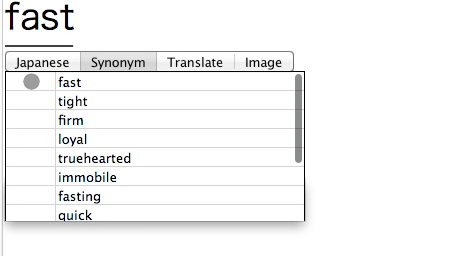
\includegraphics[width=70mm,bb=0 0 350 250]{figures/synonym.png}}
\caption{{\system}の類語変換機能の例}
\label{synonym}
\end{figure}

図\ref{image1},\ref{image2}は{\system}の画像入力の例である.
ここでは、「知らない」という入力語句について画像を検索し,入力候補として表示している.
画像が埋め込めるテキストエリアであれば画像を埋め込み,
そうでなければURLが入力される.

\begin{figure}[H]
\centerline{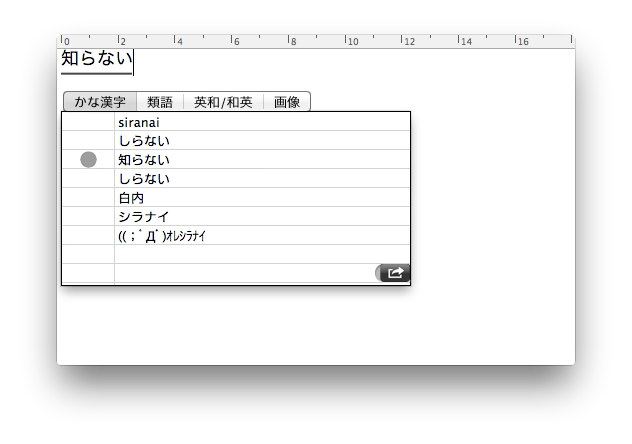
\includegraphics[width=70mm,bb=0 0 600 400]{figures/image1.png}}
\caption{{\system}で「知らない」という単語を入力した例}
\label{image1}
\end{figure}

\begin{figure}[H]
\centerline{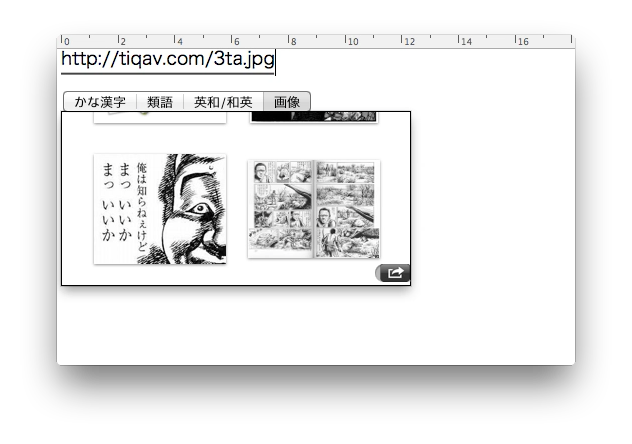
\includegraphics[width=70mm,bb=0 0 600 400]{figures/image2.png}}
\caption{{\system}の画像入力ウィンドウ}
\label{image2}
\end{figure}

{\system}を利用すると,
このような高度なテキスト編者操作も
あらゆるアプリケーションで共通に利用できる.

\subsection{テキスト入力/編集以外への応用}

本論文ではテキストエディタに絞った説明を行なったが,
IMEはユーザのすべてのキー入力を直接受け取る窓口になっているため,
キー操作をテキスト編集と関係無い仕事に割り当てることも可能である.
%
たとえばシステム音量や画面の明るさなども
{\system}から制御することが可能であり,
システムで用意されたショートカット設定などが不要になる.

\subsection{本手法の限界}

IME は,テキストエリアが実装されたアプリケーションとは個別に実装されているため,
現在の{\system}の実装ではアプリケーションの内部状態によって動作を変えたり,
アプリケーションの振る舞いを制御したりすることはできず,表に出ているテキストの編集操作しか
できない.

%
既存のシステム自体は変更せずに,皮をかぶせる形で機能を拡張す
る手法はある程度有用ではあるが,問題の根本的な解決が必要な場合には限界
がある.
%
テキスト編集の場合は根本的に解決しなければならない問題は多くな
いので,本論文の手法はとりあえず有効だといえるが,根本的な解決のために
は,テキスト入力の枠組みであるIMEに加えて,各コンピュータがテキスト編集
操作を一元化するための枠組みを用意する必要があるだろう.
